\begin{figure}[ht]
  \begin{minipage}[b]{0.48\linewidth}
    \centering
    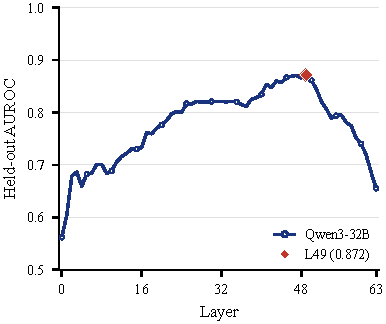
\includegraphics[width=\linewidth]{figures/fig_auroc_by_layer_32b_panel.pdf}
    \small\textbf{(a)} Held-out AUROC by layer.
  \end{minipage}
  \hfill
  \begin{minipage}[b]{0.48\linewidth}
    \centering
    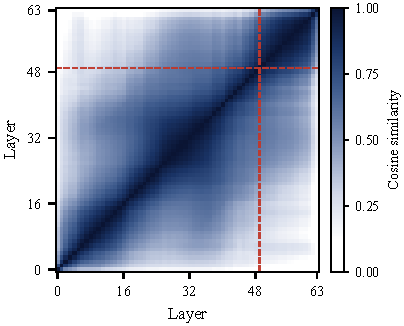
\includegraphics[width=\linewidth]{figures/fig_axis_cosine_32b_panel.pdf}
    \small\textbf{(b)} Pairwise similarity across layers.
  \end{minipage}
  \caption{\textbf{The Qwen3-32B value axis generalizes to held-out criteria.}
  \textbf{(a)} Separation strengthens through middle-to-late layers, peaking at layer 49
  (AUROC $= 0.872$; $N{=}150$ held-out conversations).
  \textbf{(b)} Pairwise cosine similarity of per-layer axis directions.
  Early (L0--3) and late (L50+) directions are nearly orthogonal (mean-dir.\ cosine $= 0.11$);
  mid--late layers (L32--54) are mutually similar (block mean $= 0.76$).
  Dashed lines mark the primary layer.}
  \label{fig:probe_eval_32b}
\end{figure}
